\documentclass[11pt]{article}

\usepackage[left=0.75in, right=0.75in, top=0.75in, bottom=0.75in]{geometry}
\usepackage{layout}
\usepackage{ucs}
\usepackage[utf8x]{inputenc}
\usepackage{titlesec}
\usepackage{graphicx}
\usepackage{amssymb}
\usepackage{amsmath}
\usepackage{dsfont}
\usepackage{float}
\usepackage{caption}
\usepackage{subcaption}
\usepackage{array}



\title{\textbf{TS217 TP}\\Communications numériques multi-porteuses\\Les système OFDM}
\author{Maxime PETERLIN - \texttt{maxime.peterlin@enseirb-matmeca.fr}\\
Gabriel VERMEULEN - \texttt{gabriel@vermeulen.email} \\\\{ENSEIRB-MATMECA, Bordeaux}}
\date{27 mars 2015}


\begin{document}

\maketitle
\tableofcontents

\newpage

\section{Introduction}

L'objectif de ce TP de communications numériques est de mettre en œuvre avec MATLAB le codage OFDM dans le cadre d'un canal Rayleigh. Nous allons ainsi simuler une chaîne de communication CP-OFDM (préfixes cycliques OFDP) et tester ses performances.

	\section{Hypothèses et paramètres de simulation}
		
		\begin{itemize}
			\item La modulation numérique est de type BPSK (symboles iid)
			\item Le temps symbole Ts est égale à 0.05 $\mu s$
			\item Le nombre de sous-porteuses totales N est égale à 128
			\item Le nombre de sous-porteuses utilisées $N_u$ est égale à 128
			\item Les symboles OFDM sont modulés et démodulés en utilisant respectivement les algorithmes IFFT et FFT
			\item Une trame OFDM contient $N_t$ = 500 symboles OFDM
			\item Le canal de propagation est tel que $h_l(p) = \sum\limites_{k=0}^{L-1} h_l[k] \delta [p-k]$, où les $h_l[k]$ sont iid et $h_l[k] ~ N_C(0, \frac{1}{L})$. On supposera que la réponse impulsionnelle (RI) du canal est invariante sur la durée d'une trame OFDM et que L $<<$ N
			\item La durée du préfixe cyclique est égale à $T_CP \geq LT_s$
			\item Le bruit $n_l[p] ~ N_C(0, \sigma_{n_l}^2$
			\item Les échantillons du signal OFDM, du canal et du bruit sont supposés décorrélés et indépendants
		\end{itemize}

	\section{Formalisme mathématique}
	
		\begin{figure}[h]
			\centering
			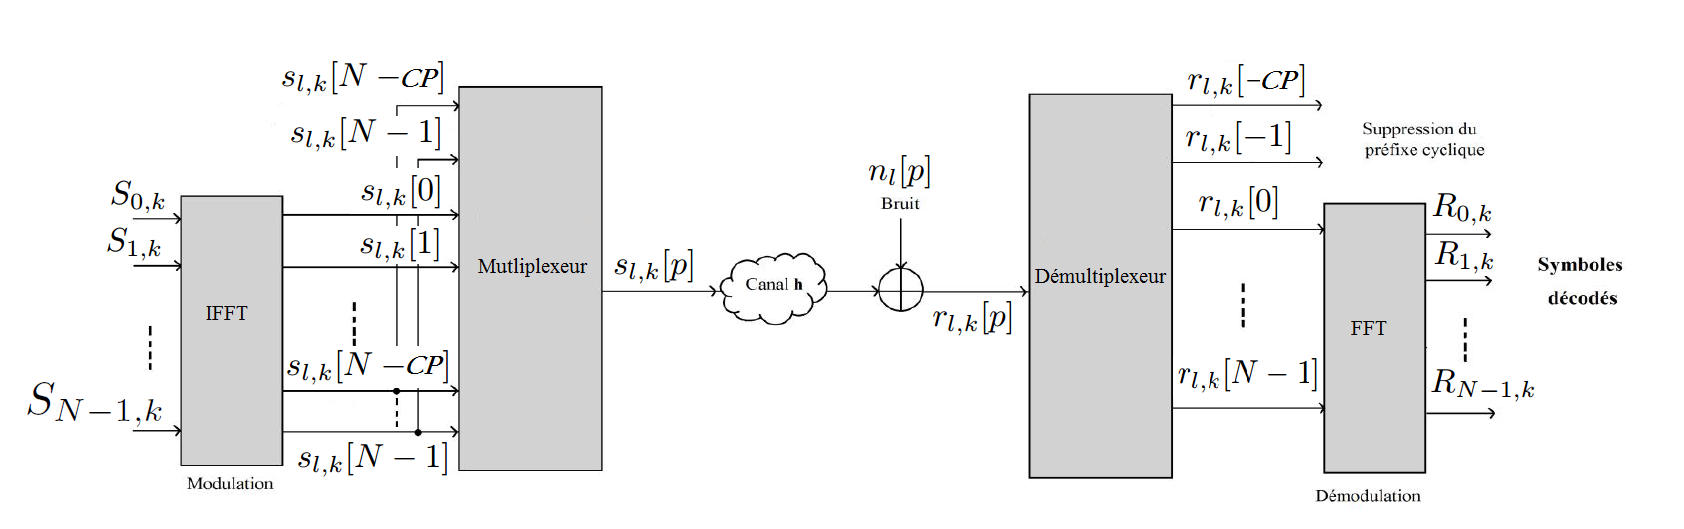
\includegraphics[scale=0.5]{img/chaine.png}
			\caption{Chaîne de communication}
			\label{chaine}
		\end{figure}
		
		Les N symboles OFDM sont notés $S_{i,k}$ avec $i\in [0, N-1]$. Les symboles sont d'abord modulés avec une transformée de Fourier inverse. On ajoute ensuite au début de la séquence les CP derniers échantillons, ce qui correspond aux préfixes cycliques. On obtient donc après multiplexage le signal suivant :\\
	\[ s_{l,k}[p] = \sum^{L-1}_{k=0}S_{l,k} . e^{\frac{j2\pi(n-CP)k}{L}} \hspace{0.5cm} avec \hspace{0.5cm} n\in [0, \cdots , N+D-1]\]
	
	Ce signal passe ensuite par le canal $h_l[p]$ et on y ajoute le bruit $n_l[p]$, tous deux définis précédemment. On obtient ainsi le signal $r_{l,k}[p]$.
	
	\[ r_{k} = H_{1}s_{k-\frac{1}{k}} + H_{2}s_{k} + n_{k} = H_{cir}s_{k} + n_{k} \]

\[
H_{cir} = 
\begin{pmatrix}
h_{0} & 0 & \cdots & 0 & h_{L-1} & \cdots & h_{1} \\
\vdots & \ddots & & & & \ddots & \vdots \\
\vdots & & \ddots & &  & & \ddots\\
h_{L-1} & & & \ddots & & & h_{L-1} \\
0 & \ddots & & & \ddots & & 0 \\
\vdots & & \ddots & & & \ddots & \vdots \\
0 & \cdots & 0 & h_{L-1} & \cdots & \cdots & h_{0} \\
\end{pmatrix} \hspace{2cm}
S_{k} =
\begin{pmatrix}
S_{l,k}[0] \\
S_{l,k}[1] \\
\vdots \\
\vdots \\
\vdots \\
S_{l,k}[N-1] \\ 
\end{pmatrix}
\]

	Après démultiplexage, chaque terme subit une transformée de Fourier permettant la démodulation et on supprime les préfixes cycliques. On obtient donc les symboles émis :
	
	\[  R_{k}[u] = H_{d}(u,u)S_{k}[u] + N_{k}[u] \hspace{0.5cm} où \hspace{0.5cm} H_{d} = \frac{1}{\sqrt{N}}\sum^{N-1}_{n=0}h_{n}e^{-\frac{j2\pi nu}{N}} \hspace{0.5cm}(\hspace{0.1cm}TF\hspace{0.1cm} du\hspace{0.1cm} canal\hspace{0.1cm}).\]
	
	
	\section{Implémentation et validation de la chaîne de communication}
	
	La chaîne de communication implémenté sous MATLAB est testée en vérifiant que le TEB est nul lorsqu'il n'y a pas de canal et pas bruit.\\
	La courbe du TEB en fonction du bruit nous permet également d'avoir une confirmation du bon fonctionnement de notre chaîne de communication.

		\begin{figure}[h]
			\centering
			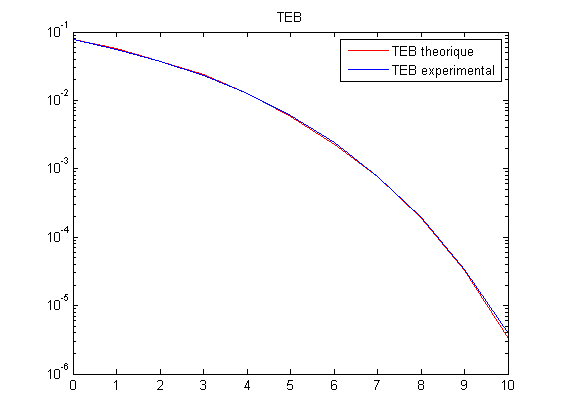
\includegraphics[scale=0.6]{img/teb.png}
			\caption{TEB en fonction du SNR}
			\label{teb}
		\end{figure}
		
		On remarque que plus le rapport signal sur bruit est important, moins le taux d'erreur binaire est élevé.
		
	\section{Implémentation d'un égaliseur par forçage à zero}
	
	Le test de l'égaliseur se fait avec L = 16 et $\sigma_{n_l}^2$.
		
		\begin{figure}[h]
			\centering
			\includegraphics[scale=0.6]{img/TEBegal.png}
			\caption{TEB en fonction du SNR}
			\label{egal}
		\end{figure}
	
	\section{Performances de la chaîne de communication}
	
		\subsection{Avec CP \geq L}
		
		\begin{figure}[h]
			\centering
			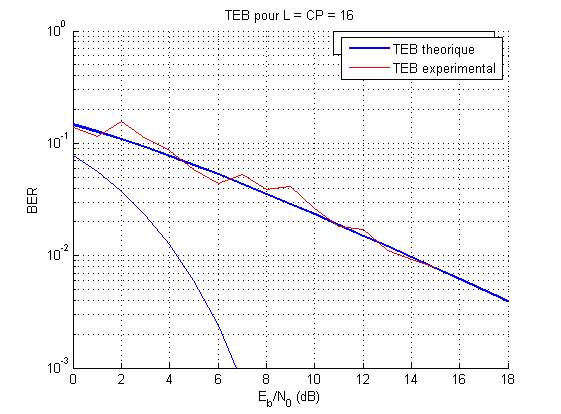
\includegraphics[scale=0.6]{img/teb1.png}
			\caption{TEB en fonction du SNR pour la nème sous-porteuse}
			\label{teb1}
		\end{figure}
		
		\subsection{Avec CP < L}

		\begin{figure}[h]
			\centering
			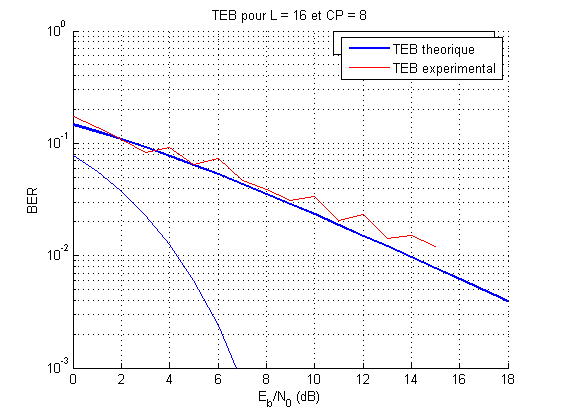
\includegraphics[scale=0.6]{img/teb2.png}
			\caption{TEB en fonction du SNR pour la nème sous-porteuse}
			\label{teb2}
		\end{figure}
		
		\section{Conclusion}
		Ce TP nous aura permis de mettre en œuvre et de tester les performances d'une modulation CP-OFDM. On retiendra que l'avantage des préfixes cycliques est de rendre la convolution du canal circulaire éliminant ainsi l'IES. Les performances de cette modulation sont meilleurs qu'une modulation OFDM classique seulement si la condition $CP \geq L$ est vérifié.
\end{document}
